% =============================================================================
% DATA 201 - Final Technical Report
% Group 5: Naman Sudan, River Roseveare-Hunt, Ishaan Shetty
% Spring 2026, San Jose State University
%
% Compile order on Overleaf: pdflatex -> bibtex -> pdflatex -> pdflatex
% Or just hit "Recompile" twice on Overleaf and the bibliography will resolve.
% =============================================================================

\documentclass[10pt,conference]{IEEEtran}

% Standard IEEE-friendly packages
\usepackage[utf8]{inputenc}
\usepackage{cite}
\usepackage{amsmath,amssymb,amsfonts}
\usepackage{algorithmic}
\usepackage{graphicx}
\usepackage{textcomp}
\usepackage{xcolor}
\usepackage{booktabs}
\usepackage{array}
\usepackage{listings}
\usepackage{url}
\usepackage{hyperref}

\hypersetup{
  colorlinks=true,
  linkcolor=blue!50!black,
  citecolor=blue!50!black,
  urlcolor=blue!50!black
}

% SQL listings setup (used in sections/06_sql_analysis.tex)
% SQL syntax styling for the listings package.
% Imported by main.tex and consumed throughout sections/06_sql_analysis.tex.

\lstdefinelanguage{SQL}{
  morekeywords={SELECT,FROM,WHERE,JOIN,LEFT,RIGHT,INNER,OUTER,FULL,CROSS,
                ON,AND,OR,NOT,IS,NULL,GROUP,BY,HAVING,ORDER,LIMIT,OFFSET,
                WITH,AS,CASE,WHEN,THEN,ELSE,END,DISTINCT,COUNT,SUM,AVG,
                MIN,MAX,ROW_NUMBER,DENSE_RANK,RANK,LAG,LEAD,OVER,
                PARTITION,EXISTS,IN,UNION,INTERSECT,EXCEPT,EXPLAIN,
                ANALYZE,CREATE,INDEX,VIEW,TABLE,INSERT,UPDATE,DELETE,
                BEGIN,COMMIT,ROLLBACK,EXTRACT,EPOCH,COALESCE,CAST,
                STRING_AGG,DATE,TIMESTAMP},
  sensitive=false,
  morecomment=[l]{\-\-},
  morestring=[b]'
}

\lstset{
  basicstyle=\ttfamily\footnotesize,
  keywordstyle=\bfseries\color{blue!60!black},
  commentstyle=\itshape\color{green!50!black},
  stringstyle=\color{purple},
  breaklines=true,
  breakatwhitespace=true,
  showstringspaces=false,
  frame=single,
  framesep=4pt,
  xleftmargin=4pt,
  language=SQL,
  captionpos=b,
  tabsize=2
}


\begin{document}

\title{Reconstructing a Multi-Stage Cyberattack with a Relational Database:\\
A 3NF Schema and SQL Analytics over the AIT-LDSv2.0 Log Corpus}

\author{
\IEEEauthorblockN{Naman Sudan, River Roseveare-Hunt, Ishaan Shetty}
\IEEEauthorblockA{Department of Applied Data Science\\
San Jose State University\\
DATA 201, Spring 2026 (Group 5)\\
\{naman.sudan, river.roseveare-hunt, ishaan.shetty\}@sjsu.edu}
}

\maketitle

\begin{abstract}
We design, load, and exercise a third normal form (3NF) relational
database over the AIT Log Data Set V2.0 (AIT-LDSv2.0), a publicly
released enterprise security log corpus that captures a simulated
multi-stage cyberattack across 22 networked hosts. The
\texttt{russellmitchell} testbed slice contains 295{,}243 raw log lines
across eight sources and 61{,}862 ground-truth attack labels spanning
seven kill-chain phases. Our schema decomposes a heterogeneous mix of
YAML, key-value \texttt{auditd}, and JSONL data into 22 normalized
tables organized into three domains (host inventory, audit events,
attack labels), enforced by primary and foreign key constraints in
PostgreSQL 16. We articulate the normalization journey from staging
tables (which preserve source-faithful 1NF violations) to 3NF using
surrogate keys, lookup tables, and supertype/subtype decomposition of
\texttt{auditd} records. On top of the loaded database we present a portfolio of 23 SQL query
items (7 basic and 16 advanced, committed across 6 basic and 13
advanced \texttt{.sql} files) that cover subqueries, common table
expressions, window functions, multi-table joins of three or more
tables, performance indexing with \texttt{EXPLAIN ANALYZE}, and a
saved view. The portfolio answers concrete attack-investigation
questions: from baseline service activity, to detection-rule
effectiveness, to a CTE-and-window-function reconstruction of the
privilege-escalation sequence on a single host that joins seven
tables.
We further demonstrate an indexing improvement on the incident-response
access pattern (composite index
\texttt{idx\_audit\_event\_host\_timestamp}, execution time 1.462~ms to
0.640~ms, buffers 141 to 33), a saved view
\texttt{v\_privilege\_escalation\_timeline} that collapses an
eight-table cross-domain join into a single virtual relation, and an
interactive Streamlit dashboard exposing nine visualizations (one
filter-driven KPI panel and eight story panels) directly bound to
these queries. Our findings show that exfiltration-related labels
dominate the corpus by line count (53{,}000+ lines across two log
sources), while privilege escalation, the most operationally critical
phase, leaves only 82 labeled lines but spans five distinct log
sources, illustrating why a relational schema with cross-source joins
is more diagnostic than any single log file in isolation.
\end{abstract}

\section{Introduction}
\label{sec:introduction}

\subsection{Motivation}
Modern enterprise networks emit log streams from a heterogeneous mix of
systems: web servers, audit daemons, virtual private network endpoints,
name-resolution services, and authentication subsystems. Security
operations teams must reason across these streams to detect attacker
activity, attribute events to a kill-chain phase, and reconstruct a
timeline after the fact. In practice, the work is hampered because
each log type lives in its own format, storage location, and tool. A
relational database offers a single substrate where structured queries
can join evidence across sources and ground-truth labels.

This project takes a published, labeled, multi-host security log corpus
\cite{landauer2022maintainable, ait2024dataset} and asks whether a
single PostgreSQL database in third normal form can support a
meaningful cross-log analysis of a real multi-stage attack. The dataset
ships with attacker ground truth: every log line that participates in
the simulated attack chain is labeled with one or more attack-phase
identifiers, allowing us to quantify both detection coverage and the
cost of false positives.

\subsection{Problem and Research Gap}
The AIT-LDSv2.0 corpus is large and heterogeneous: 295{,}243 log lines
from eight sources on the \texttt{russellmitchell} testbed, with
61{,}862 labeled attack events across seven kill-chain phases. Most
published exploration of the dataset treats each log file
independently, or flattens the entire corpus into a single denormalized
table, losing the relational structure that makes cross-source queries
cheap. We close that gap by:
\begin{itemize}
  \item Designing a 3NF schema that explicitly separates the host
    inventory, audit event, and attack-label domains while preserving
    cross-domain provenance and foreign keys.
  \item Implementing a reproducible ETL from raw files through staging
    tables into the final 3NF schema, with Alembic-managed migrations.
  \item Demonstrating that the resulting database supports analytical
    SQL expressive enough to reconstruct attack sequences and to
    compare detection-rule effectiveness across log sources.
\end{itemize}

\subsection{Scope and Story Arc}
Across the eight log sources in the \texttt{russellmitchell} slice, the
attack chain traces a coherent sequence: a web foothold on
\texttt{intranet\_server}'s \texttt{access.log.2} during the
\texttt{initial\_access} phase, a \texttt{su} then
\texttt{sudo cat /etc/shadow} chain captured by the host's
\texttt{audit.log} during the \texttt{privilege\_escalation} phase,
and a DNS-tunneling \texttt{put} service on \texttt{internal\_share}
during the \texttt{exfiltration} phase roughly nine hours later. The
narrative through this report follows the lead-in plus climax pair on
\texttt{intranet\_server}; the exfiltration phase is reported as
``what happened next'' in Section~\ref{sec:conclusion} and reproduced
in the appendix.

\subsection{Project Goals}
The project has four explicit deliverables, each of which is reflected
in a section of this report:
\begin{enumerate}
  \item A normalized relational schema with documented PK/FK and
    normalization decisions (Section~\ref{sec:schema}).
  \item A reproducible PostgreSQL load pipeline with row-count
    verification (Section~\ref{sec:dbsetup}).
  \item A portfolio of 23 SQL query items (7 basic and 16 advanced,
    spread across 6 basic and 13 advanced \texttt{.sql} files) that
    answer concrete attack-investigation questions, including
    indexing/\texttt{EXPLAIN} performance work and a saved view
    (Section~\ref{sec:sql}).
  \item An interactive dashboard with nine visualizations that
    surfaces the query results to a non-SQL audience
    (Section~\ref{sec:dashboard}).
\end{enumerate}

\section{Dataset and Data Processing}
\label{sec:dataset}

\subsection{Source}
We use the \emph{russellmitchell} testbed slice of the AIT Log Data Set V2.0
(AIT-LDSv2.0) \cite{landauer2022maintainable, ait2024dataset}. The corpus
simulates a four-day attack window (January 21 to 25, 2022, UTC) on a 22-host
enterprise network running a mix of Ubuntu and Debian distributions. The
dataset is publicly available under a permissive research license at the
URL given in the bibliography entry.

\subsection{Scale and Heterogeneity}
The \emph{russellmitchell} slice contains 295{,}243 raw log lines across
eight source files on five hosts and 61{,}862 ground-truth attack labels
spanning seven kill-chain phases (reconnaissance, initial access, privilege
escalation, lateral movement, exfiltration, command and control,
persistence). Forty-six unique attributes appear across log types. The
corpus deliberately mixes formats to mirror real environments:
\begin{itemize}
  \item \textbf{YAML}: \texttt{processing/config/servers.yaml} encodes the
    host inventory with multi-valued fields (\texttt{groups},
    \texttt{fqdns}, \texttt{ipv4\_addresses}, \texttt{ipv6\_addresses}).
  \item \textbf{Linux \texttt{auditd}} key-value records: 3{,}048 events
    across two hosts (\texttt{intranet\_server} and
    \texttt{internal\_share}), capturing PAM authentication, service
    lifecycle, login, and command-execution traces.
  \item \textbf{JSONL labels}: 8 files containing per-line label
    annotations across 5 hosts, totalling 61{,}862 labeled events with 22
    distinct label types.
  \item \textbf{Apache combined-log}, \textbf{OpenVPN syslog},
    \textbf{dnsmasq}, \textbf{system auth} formats are present in the
    corpus but out of scope for the iteration documented here.
\end{itemize}

\subsection{Why This Dataset}
Two properties make AIT-LDSv2.0 a strong fit for a relational-database
project. First, the corpus is \emph{inherently denormalized}: multi-valued
fields, key-value blobs, and overlapping record types force a real
normalization exercise rather than a perfunctory 1NF pass. Second, the
ground-truth labels enable cross-source queries with verifiable answers:
``which detection rules fire on the privilege escalation phase'' is a
question with a numeric answer the database can compute, not a subjective
judgment call.

\subsection{Data Quality and Cleaning}
The raw corpus has three classes of cleaning concerns that we document and
address explicitly during ETL (Section \ref{sec:dbsetup}):
\begin{enumerate}
  \item \textbf{Multi-valued fields} (1NF violations) in the host YAML and
    in the \texttt{auditd} \texttt{msg} blob. We preserve them in staging
    tables (source-faithful) and decompose them into child tables during
    the staging-to-3NF transformation.
  \item \textbf{Sentinel values}: \texttt{auid}/\texttt{ses}=4294967295
    represent ``unset.'' We preserve the raw value but document its
    semantics so query authors do not treat it as a real session.
  \item \textbf{Sparse columns from heterogeneous record types}: a single
    \texttt{auditd} log file contains $\geq 8$ structurally different
    record types (LOGIN, SYSCALL, AVC, PROCTITLE, PAM events, etc.). A
    flat-table representation would have $\sim 80\%$ NULL columns. We
    apply supertype/subtype decomposition (Section \ref{sec:schema}) to
    push subtype-specific attributes out of the supertype.
\end{enumerate}

\subsection{Coverage Summary}
Table~\ref{tab:source-coverage} groups the eight \texttt{russellmitchell}
source files by host and gives the labeled-line count and the dominant
attack phase recorded against each one. The table makes the
foothold-to-escalate story on \texttt{intranet\_server} visible at a
glance, and reminds the reader that the exfiltration evidence on
\texttt{internal\_share} also belongs to the same attack chain even
though it lives on a different host.

\begin{table}[htbp]
\caption{Labeled-line coverage by source file. The first six rows are the
audit and host-side evidence; the final row is the bulk DNS-tunneling
channel that drives the corpus-wide line count.}
\label{tab:source-coverage}
\centering
\footnotesize
\setlength{\tabcolsep}{4pt}
\begin{tabular}{llrl}
\toprule
\textbf{Host} & \textbf{Source log} & \textbf{Lines} & \textbf{Dominant phase} \\
\midrule
intranet\_server & access.log.2 & 7{,}691           & initial\_access \\
intranet\_server & auth.log     & 8                 & privilege\_escalation \\
intranet\_server & audit.log    & 9                 & privilege\_escalation \\
internal\_share  & audit.log    & 2                 & exfiltration \\
inet-firewall    & dnsmasq.log  & 12                & privilege\_escalation \\
monitoring       & cpu.log      & 49                & privilege\_escalation \\
\midrule
internal\_share  & dns.log      & $\approx$53{,}000 & exfiltration \\
\bottomrule
\end{tabular}
\end{table}

\section{Schema and Normalization}
\label{sec:schema}

The relational design has three domains and 22 tables. The ER/EER diagram
in Figure \ref{fig:eer} shows the full schema; primary keys are underlined
and foreign keys are rendered as directed edges. The normalization journey
is documented in detail in \texttt{docs/schema/normalization\_raw\_to\_3nf.md}
and the relation catalog in \texttt{docs/schema/data\_model\_3nf.md}; this
section summarizes the design rationale.

\begin{figure*}[htbp]
  \centering
  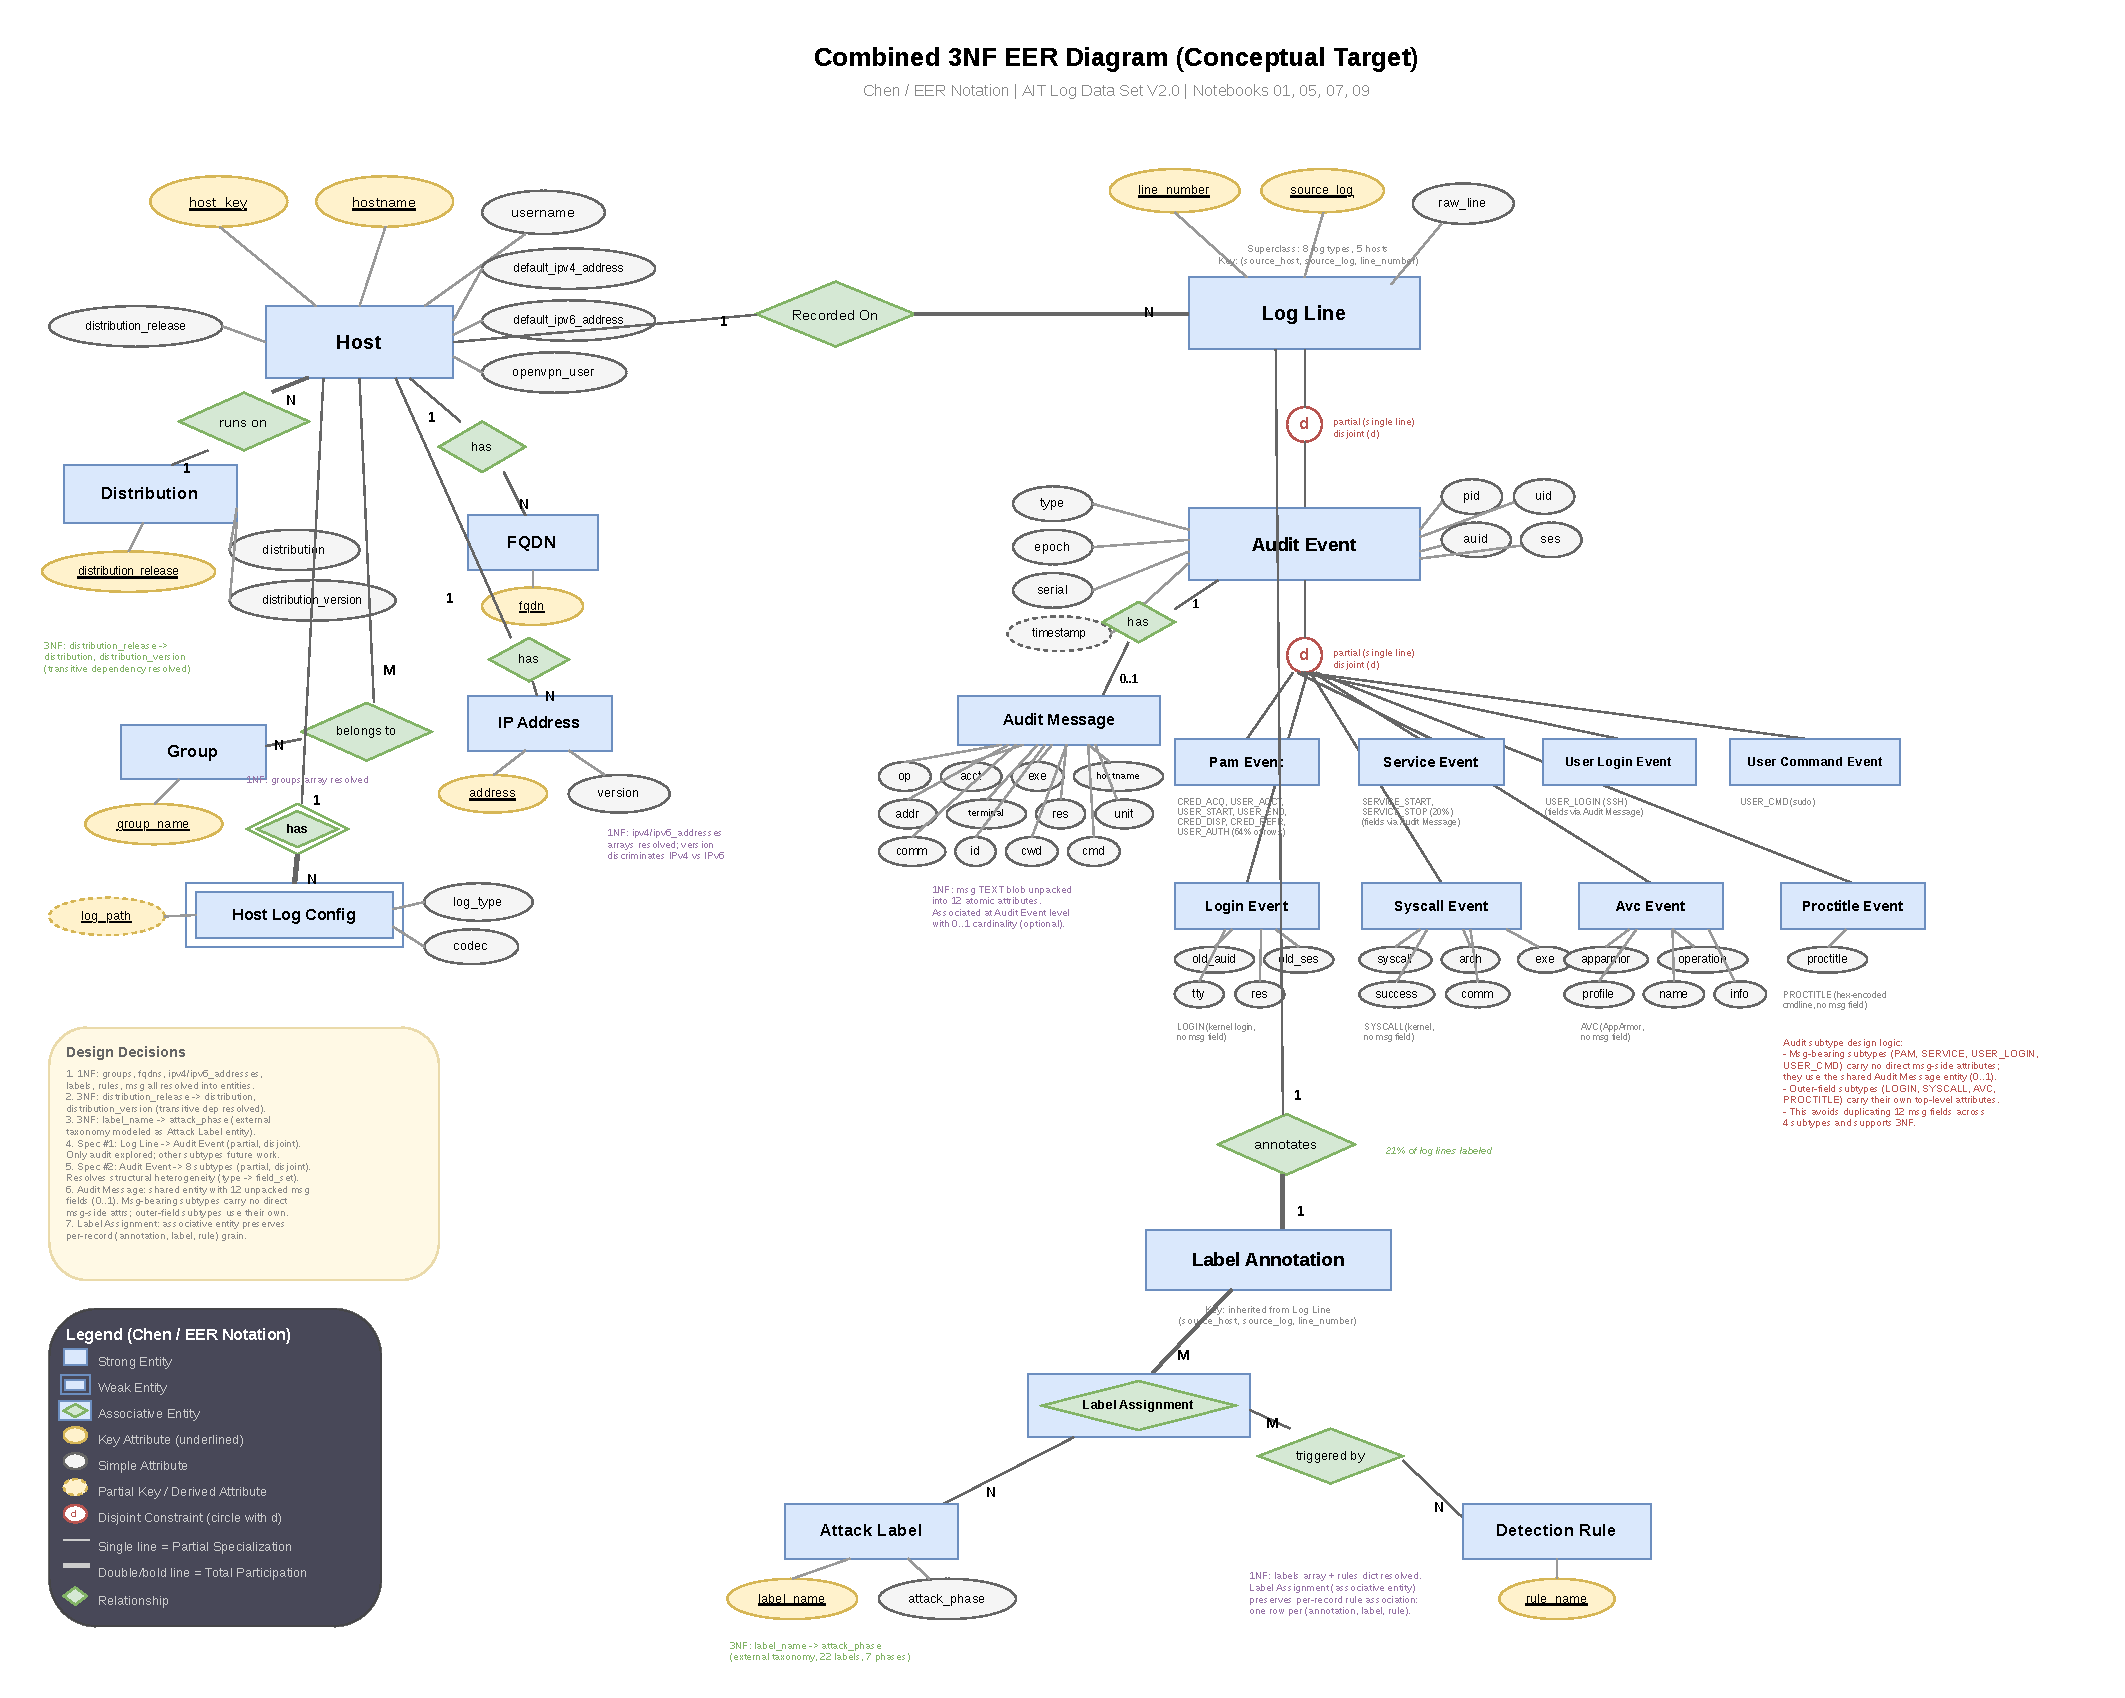
\includegraphics[width=0.95\textwidth]{figures/eer_3nf_combined.pdf}
  \caption{Final 3NF EER schema: 22 tables across host inventory (7),
    audit events (10), and attack labels (5) domains. Surrogate primary
    keys (SERIAL) are used throughout to keep foreign-key columns narrow
    across the join graph.}
  \label{fig:eer}
\end{figure*}

\subsection{Domain 1: Host Inventory (7 tables)}
The host domain captures the testbed inventory. The core entity is
\texttt{host}, with row grain ``one row per machine'' and 22 rows total.
Three multi-valued attributes (\texttt{groups}, \texttt{fqdns},
\texttt{ipv4\_addresses}, \texttt{ipv6\_addresses}) become 1NF child
tables (\texttt{host\_group}, \texttt{host\_fqdn}, \texttt{host\_ipv4},
\texttt{host\_ipv6}) with composite primary keys. The transitive
dependency
\texttt{distribution\_release} $\rightarrow$
\{\texttt{distribution}, \texttt{distribution\_version}\}
is removed by the 3NF lookup table \texttt{os\_release} (2 rows: bionic
and stretch). The \texttt{logs} composite multi-valued field becomes
\texttt{host\_log\_config} (66 rows, 1 to 9 configs per host).

\subsection{Domain 2: Audit Events (10 tables)}
The audit domain demonstrates supertype/subtype decomposition. The
supertype \texttt{audit\_event} (3{,}048 rows) carries the attributes
common to every \texttt{auditd} record (\texttt{event\_id},
\texttt{host\_id}, \texttt{type}, \texttt{epoch}, \texttt{timestamp},
\texttt{pid}, \texttt{uid}, \texttt{auid}, \texttt{ses},
\texttt{line\_number}, \texttt{raw\_line}). Two classes of subtypes
extend it:

\begin{itemize}
  \item \textbf{Msg-bearing subtypes}: \texttt{audit\_pam\_event},
    \texttt{audit\_service\_event}, \texttt{audit\_user\_login\_event},
    \texttt{audit\_user\_cmd\_event}. The semantic content for these
    subtypes lives inside the \texttt{msg=` ... '} key-value blob in the
    raw line. We resolve this 1NF violation by parsing the blob into 12
    atomic columns in \texttt{audit\_message} (2{,}614 rows), which holds
    a 0..1 relationship with \texttt{audit\_event}.
  \item \textbf{Outer-field subtypes}: \texttt{audit\_login\_event},
    \texttt{audit\_syscall\_event}, \texttt{audit\_avc\_event},
    \texttt{audit\_proctitle\_event}. These record types carry their
    semantic content as top-level fields rather than inside \texttt{msg};
    the subtype tables hold those fields directly.
\end{itemize}

The decomposition turns a hypothetical flat ``audit\_line'' table with
$\sim 44$ columns and 80\% NULL density into a supertype + 9 sparse
subtype tables with full population per subtype. The cost is more joins
in queries; the benefit is correct cardinality, query-planner statistics,
and a cleaner mental model.

\subsection{Domain 3: Attack Labels (5 tables)}
The label domain links log lines to attacker activity. The grain is one
row per \emph{labeled} log line, identified by the natural key
(\texttt{source\_host}, \texttt{source\_log}, \texttt{line\_number}).
\texttt{labeled\_line} (61{,}862 rows) is the line-level fact table;
\texttt{labeled\_line\_label} is the M:N junction connecting lines to
labels; \texttt{labeled\_line\_rule} captures which detection rule
generated each label (an event can be labeled by multiple rules). The
taxonomy is normalized into two lookup tables: \texttt{attack\_label}
(22 rows: distinct label names) and \texttt{attack\_phase} (7 rows:
kill-chain phases), with a 1:N relationship from phase to label.

\subsection{Normalization Decisions Worth Calling Out}
Three decisions are explicit project rules rather than mechanical
applications of the normalization algorithm:
\begin{enumerate}
  \item \textbf{Surrogate keys throughout.} Every entity has a SERIAL
    primary key, even when the natural key (e.g. \texttt{host\_key},
    \texttt{(source\_host, source\_log, line\_number)}) is unique. This
    keeps foreign-key columns narrow (\texttt{INT} rather than
    \texttt{VARCHAR(50)}) and decouples domain-key changes from join
    indexes. The natural key is preserved as a \texttt{UNIQUE} constraint.
  \item \textbf{Provenance preserved on the supertype.}
    \texttt{audit\_event} carries the original \texttt{raw\_line} TEXT
    even after the parsed columns are populated. This is a deliberate
    space cost in exchange for reproducibility: we can re-derive any
    parsed field from the raw text if a downstream bug is found.
  \item \textbf{One pragmatic 1NF exception.} \texttt{host\_log\_config}
    has an \texttt{add\_field\_json TEXT} column that retains the JSON
    payload of optional log-specific fields. Rather than create a
    polymorphic child table per log type (high schema cost, low query
    value), we leave the JSON opaque and query it with PostgreSQL
    \texttt{jsonb\_path\_query} when needed. The exception is documented
    and the column is unused by the queries in Section \ref{sec:sql}.
\end{enumerate}

\subsection{3NF Claim}
For each non-key attribute in every relation, we verified that the
attribute depends only on the primary key (no partial dependencies, as
all primary keys are atomic SERIAL surrogates) and that it does not
transitively depend on another non-key attribute. The two textbook
candidates for transitive dependency in the source data
(\texttt{distribution\_release} $\rightarrow$ \texttt{distribution},
\texttt{distribution\_version}) and the lookup-style relationship
(\texttt{label\_name} $\rightarrow$ \texttt{phase\_name}) are removed
by promoting them into separate lookup tables (\texttt{os\_release}
and \texttt{attack\_phase}, respectively). The one
documented exception is \texttt{host\_log\_config.add\_field\_json},
which is a TEXT blob carrying log-type-specific configuration values.
We treat the column as opaque (queried only with PostgreSQL JSON
functions when needed) rather than synthesizing a polymorphic child
table. The exception is documented in
\texttt{docs/schema/data\_model\_3nf.md} and the column is unused by
any query in Section~\ref{sec:sql}.

\section{Database Setup and Loading}
\label{sec:dbsetup}

\subsection{Stack}
We use PostgreSQL 16 \cite{postgresql} running inside a single Docker
container defined in \texttt{docker-compose.yml} \cite{docker}. Schema
migrations are managed by Alembic \cite{alembic} so that any team
member can rebuild the database from a clean state with a single
command. Application code is Python 3.12 with SQLAlchemy ORM models
for parsing and loading.

\subsection{Repository Layout}
\begin{lstlisting}[basicstyle=\ttfamily\scriptsize, frame=none, language={}]
data-201-security-log-analysis/
|-- alembic/              schema migrations
|-- docker-compose.yml    Postgres 16
|-- src/
|   |-- models/           SQLAlchemy models
|   |-- parsers/          raw -> dict parsers
|   |-- loaders/          dict -> row loaders
|   `-- dashboard/        Streamlit app + db.py
|-- sql/
|   |-- 3nf/              per-table CREATE TABLE
|   |-- 3nf/_indexes.sql  canonical index DDL
|   |-- 3nf/_views.sql    canonical view DDL
|   |-- queries/basic/    6 basic .sql files
|   `-- queries/advanced/ 13 advanced .sql files
|-- notebooks/            10 exploration nbs
|-- docs/                 schema, ERD, findings
`-- report/               this report
\end{lstlisting}

\subsection{Reproducible Load}
The full load runs in five commands from a clean clone of the
repository:

\begin{lstlisting}[language=bash, basicstyle=\ttfamily\small, frame=single]
docker compose up -d                  # Postgres on :5432
python -m venv venv && source venv/bin/activate
pip install -r requirements.txt
alembic -c alembic/alembic.ini upgrade head
python -m src.loaders.run_all
\end{lstlisting}

The migration chain creates 22 tables across staging and 3NF schemas;
the loader script reads the raw \texttt{russellmitchell} files, runs
the parsers in \texttt{src/parsers/}, and inserts rows in dependency
order (host inventory first, then audit events, then attack labels).
The loader is idempotent: re-running against an already-loaded database
truncates and re-inserts each table inside a transaction, so the
output is reproducible regardless of starting state.

\subsection{Migration Head and Schema Objects}
After \texttt{alembic upgrade head} the database carries revision
\texttt{742e860d116f}, which adds two analytical objects on top of the
22-table 3NF base:
\begin{itemize}
  \item Composite index
    \texttt{idx\_audit\_event\_host\_timestamp} on
    \texttt{audit\_event(host\_id, timestamp)}, the index that powers
    the incident-response speedup documented in
    Section~\ref{sec:explain}.
  \item Saved view \texttt{v\_privilege\_escalation\_timeline}, an
    eight-table cross-domain join filtered to
    \texttt{attack\_phase.phase\_name = 'privilege\_escalation'} and
    aggregated with \texttt{string\_agg}, used by both the dashboard
    and the deep-dive query in Section~\ref{sec:view}.
\end{itemize}
A teammate can verify that both objects are present with one psql
command:

\begin{lstlisting}[language=bash, basicstyle=\ttfamily\small, frame=single]
docker exec security-logs-dev psql -U security_logs_user \
  -d security_logs \
  -c "SELECT version_num FROM alembic_version;" \
  -c "SELECT indexname FROM pg_indexes
      WHERE tablename = 'audit_event'
      ORDER BY indexname;" \
  -c "SELECT viewname FROM pg_views
      WHERE schemaname = 'public';"
\end{lstlisting}

Expected output: \texttt{version\_num = 742e860d116f},
\texttt{idx\_audit\_event\_host\_timestamp} appears in the index list,
and \texttt{v\_privilege\_escalation\_timeline} appears in the view
list.

\subsection{Final Row Counts}
Table~\ref{tab:rowcounts} reports the final loaded row counts (verified
2026-05-01 against the loaded database). Total across all 22 tables is
roughly 439{,}998 rows. The largest single table is
\texttt{labeled\_line\_rule} (184{,}651 rows: a per-rule annotation on
labeled lines), closely followed by \texttt{labeled\_line\_label}
(184{,}517 rows: the line-to-label many-to-many junction).

\begin{table}[htbp]
\caption{Final loaded row counts by domain (verified 2026-05-01).}
\label{tab:rowcounts}
\centering
\begin{tabular}{lll}
\toprule
\textbf{Domain} & \textbf{Table} & \textbf{Rows} \\
\midrule
Host inventory   & host                       & 22       \\
                 & host\_group                & 63       \\
                 & host\_fqdn                 & 20       \\
                 & host\_ipv4                 & 24       \\
                 & host\_ipv6                 & 24       \\
                 & host\_log\_config          & 66       \\
                 & os\_release                & 2        \\
\midrule
Audit events     & audit\_event               & 3{,}048  \\
                 & audit\_message             & 2{,}614  \\
                 & audit\_pam\_event          & 2{,}055  \\
                 & audit\_service\_event      & 555      \\
                 & audit\_login\_event        & 410      \\
                 & audit\_user\_login\_event  & 3        \\
                 & audit\_user\_cmd\_event    & 1        \\
                 & audit\_syscall\_event      & 8        \\
                 & audit\_avc\_event          & 8        \\
                 & audit\_proctitle\_event    & 8        \\
\midrule
Attack labels    & labeled\_line              & 61{,}862 \\
                 & labeled\_line\_label       & 184{,}517 \\
                 & labeled\_line\_rule        & 184{,}651 \\
                 & attack\_label              & 22       \\
                 & attack\_phase              & 7        \\
\midrule
\textbf{Total}   &                            & \textbf{$\approx$439{,}998} \\
\bottomrule
\end{tabular}
\end{table}

\subsection{Integrity Verification}
After load we run a small set of integrity checks. The two most
load-bearing checks are the orphan-FK count on \texttt{audit\_event}
and the cross-domain consistency check between \texttt{labeled\_line}
and \texttt{audit\_event} for rows where the labeled log is
\texttt{audit.log}. Both return zero on the current database.

\begin{lstlisting}[language=SQL,basicstyle=\ttfamily\scriptsize]
-- Every audit_event references a real host (FK consistency).
SELECT COUNT(*) AS orphans
FROM audit_event ae
LEFT JOIN host h ON h.host_id = ae.host_id
WHERE h.host_id IS NULL;
-- => 0 orphans

-- Every labeled_line line_number that targets audit.log lands
-- inside its host's audit_event range.
SELECT COUNT(*) AS unmatched
FROM labeled_line ll
WHERE ll.source_log = 'audit.log'
  AND NOT EXISTS (
    SELECT 1 FROM audit_event ae
    JOIN host h ON h.host_id = ae.host_id
    WHERE h.host_key   = ll.source_host
      AND ae.line_number = ll.line_number
  );
-- => 0 unmatched

-- Subtype coverage: every audit_event has exactly one subtype row.
WITH subtype_sum AS (
  SELECT
    (SELECT COUNT(*) FROM audit_pam_event)
  + (SELECT COUNT(*) FROM audit_service_event)
  + (SELECT COUNT(*) FROM audit_user_login_event)
  + (SELECT COUNT(*) FROM audit_user_cmd_event)
  + (SELECT COUNT(*) FROM audit_login_event)
  + (SELECT COUNT(*) FROM audit_syscall_event)
  + (SELECT COUNT(*) FROM audit_avc_event)
  + (SELECT COUNT(*) FROM audit_proctitle_event)
    AS subtype_total
)
SELECT (SELECT COUNT(*) FROM audit_event) AS total_events,
       subtype_total AS sum_of_subtypes
FROM   subtype_sum;
-- => total_events = sum_of_subtypes = 3,048
\end{lstlisting}

The third check (subtype-coverage equality) is the practical proof
that the supertype/subtype decomposition described in
Section~\ref{sec:schema} is total and disjoint, which is the property
that lets the report claim ``every audit event is exactly one
subtype.''

\section{SQL Analysis and Results}
\label{sec:sql}

The query portfolio contains thirteen analytic queries (six basic and seven
advanced) plus one performance-tuned query and one persisted view. Together
they cover five SQL categories called out by the project rubric: subqueries,
common table expressions (CTEs), window functions, multi-table joins
($\geq 3$ tables), and indexing / \texttt{EXPLAIN} performance work. Every
query is committed in the project repo under \texttt{sql/queries/} with the
naming convention \texttt{<owner>\_<short\_name>.sql}.

For each query we present the domain question, the SQL, a result snapshot,
and a one-paragraph insight. Result snapshots in this report are
PostgreSQL output exported from \texttt{psql} or rendered from the
Streamlit dashboard.

\subsection{Methodology}
All queries run against the loaded database documented in
Section~\ref{sec:dbsetup}. Each query is reproducible: a reader who has
followed the load instructions can paste any \texttt{SELECT} below into
their \texttt{psql} session and obtain the same result. Where helpful we
note the technique label (CTE, window function, etc.) so the rubric
mapping is unambiguous.

% =========================================================================
\subsection{Basic Queries}
% =========================================================================

\subsubsection{B1 (River): Labeled lines per source host}
\textbf{Question.} Which hosts contribute the most labeled attack
evidence?

\begin{lstlisting}[language=SQL]
SELECT source_host,
       COUNT(*) AS labeled_line_count
FROM labeled_line
GROUP BY source_host
ORDER BY labeled_line_count DESC;
\end{lstlisting}

% TODO: insert result snapshot at figures/q_b1_result.png
\textbf{Insight.} % TBD: river to add a 2-3 sentence interpretation.
The dominant host (by labeled-line count) frames the rest of the analysis.

% -------------------------------------------------------------------------
\subsubsection{B2 (River): Attack labels per phase}
\textbf{Question.} How many distinct labels does each attack phase carry?
\begin{lstlisting}[language=SQL]
SELECT ap.phase_name,
       COUNT(al.label_id) AS label_count
FROM attack_phase ap
FULL OUTER JOIN attack_label al ON al.phase_id = ap.phase_id
GROUP BY ap.phase_id, ap.phase_name
ORDER BY label_count DESC;
\end{lstlisting}
% TODO: insert result snapshot at figures/q_b2_result.png
\textbf{Insight.} % TBD river: which phases have the richest taxonomy?

% -------------------------------------------------------------------------
\subsubsection{B3 (River): Audit-event count per host}
\textbf{Question.} Which hosts produce \texttt{auditd} traces, and how
many?

\begin{lstlisting}[language=SQL]
SELECT h.hostname,
       h.host_key,
       COUNT(ae.event_id) AS event_count
FROM host h
INNER JOIN audit_event ae ON ae.host_id = h.host_id
GROUP BY h.host_id, h.hostname, h.host_key
ORDER BY event_count DESC;
\end{lstlisting}
% TODO: insert result snapshot at figures/q_b3_result.png
\textbf{Insight.} % TBD river: confirms only two hosts have audit logs in
% the russellmitchell slice.

% -------------------------------------------------------------------------
\subsubsection{B4 (Ishaan): Labeled lines per attack phase}
\textbf{Question.} How heavily is each phase represented in the labeled
data?
\begin{lstlisting}[language=SQL]
SELECT ap.phase_name, COUNT(*) AS labeled_lines
FROM attack_phase ap
JOIN attack_label al  ON al.phase_id  = ap.phase_id
JOIN labeled_line_label lll ON lll.label_id = al.label_id
GROUP BY ap.phase_name
ORDER BY labeled_lines DESC;
\end{lstlisting}
% TODO: insert result snapshot at figures/q_b4_result.png
\textbf{Insight.} % TBD ishaan: exfiltration dominates by line count.

% -------------------------------------------------------------------------
\subsubsection{B5 (Ishaan): Top-10 detection rules}
\textbf{Question.} Which rules contribute the most labels?
\begin{lstlisting}[language=SQL]
SELECT rule_name, COUNT(*) AS times_used
FROM labeled_line_rule
GROUP BY rule_name
ORDER BY times_used DESC
LIMIT 10;
\end{lstlisting}
% TODO: insert result snapshot at figures/q_b5_result.png
\textbf{Insight.} % TBD ishaan: dnsteal.domain.match dominates.

% -------------------------------------------------------------------------
\subsubsection{B6 (Naman): Service activity baseline}
\textbf{Question.} What is the baseline service activity on monitored
hosts? Establishing the baseline lets us see why one stop/start pair
later stands out as anomalous.
\begin{lstlisting}[language=SQL]
SELECT h.host_key,
       am.unit AS service_name,
       SUM(CASE WHEN ae.type = 'SERVICE_START' THEN 1 ELSE 0 END) AS starts,
       SUM(CASE WHEN ae.type = 'SERVICE_STOP'  THEN 1 ELSE 0 END) AS stops
FROM audit_event ae
JOIN audit_service_event ase ON ase.event_id = ae.event_id
JOIN audit_message am        ON am.event_id  = ae.event_id
JOIN host h                  ON h.host_id    = ae.host_id
GROUP BY h.host_key, am.unit
ORDER BY h.host_key,
         SUM(CASE WHEN ae.type = 'SERVICE_START' THEN 1 ELSE 0 END)
       + SUM(CASE WHEN ae.type = 'SERVICE_STOP'  THEN 1 ELSE 0 END) DESC;
\end{lstlisting}
% TODO: insert result snapshot at figures/q_b6_result.png
\textbf{Insight.} The query returns 33 (host, service) rows.
\texttt{phpsessionclean} dominates \texttt{intranet\_server} with 384
events. The \texttt{put} service on \texttt{internal\_share}, with a
single start and a single stop amid hundreds of routine cron-driven
service events, is a strong candidate for further investigation. This
exact pair is the exfiltration service confirmed by the attack labels.

% =========================================================================
\subsection{Advanced Queries}
% =========================================================================

\subsubsection{A1 (Ishaan): Distinct event types touching labeled hosts (Subquery)}
\textbf{Category.} Subquery (\texttt{EXISTS}).\\
\textbf{Question.} Which audit event types appear on hosts that have at
least one labeled log line?
\begin{lstlisting}[language=SQL]
SELECT DISTINCT e.type
FROM audit_event e
WHERE EXISTS (
  SELECT 1
  FROM host h
  JOIN labeled_line ll ON ll.source_host = h.host_key
  WHERE h.host_id = e.host_id
);
\end{lstlisting}
% TODO: insert result snapshot at figures/q_a1_result.png
\textbf{Insight.} % TBD ishaan: confirms which event types coexist with
% the attack-labeled lines.

% -------------------------------------------------------------------------
\subsubsection{A2 (River): Cross-host distribution of labeled lines (multi-CTE + CROSS JOIN)}
\textbf{Category.} CTE.\\
\textbf{Question.} What share of labeled lines comes from each
(host, log) pair?

\begin{lstlisting}[language=SQL]
WITH per_source AS (
    SELECT source_host, source_log, COUNT(*) AS line_count
    FROM labeled_line
    GROUP BY source_host, source_log
),
total AS (
    SELECT SUM(line_count) AS total_count FROM per_source
)
SELECT ps.source_host,
       ps.source_log,
       ps.line_count,
       ROUND(100.0 * ps.line_count / t.total_count, 2)
         AS pct_of_all_labeled
FROM per_source ps
CROSS JOIN total t
ORDER BY ps.line_count DESC;
\end{lstlisting}
% TODO: insert result snapshot at figures/q_a2_result.png
\textbf{Insight.} % TBD river: shows the long-tail concentration.

% -------------------------------------------------------------------------
\subsubsection{A3 (Ishaan): Busiest day per host (Window function)}
\textbf{Category.} Window function (\texttt{RANK}~\texttt{OVER PARTITION}).\\
\textbf{Question.} On what day did each host generate the most events?

\begin{lstlisting}[language=SQL]
SELECT h.host_key,
       DATE(e.timestamp) AS event_date,
       COUNT(*) AS events_that_day,
       RANK() OVER (
           PARTITION BY h.host_key
           ORDER BY COUNT(*) DESC
       ) AS day_rank_for_host
FROM audit_event e
JOIN host h ON h.host_id = e.host_id
GROUP BY h.host_key, DATE(e.timestamp)
ORDER BY h.host_key, day_rank_for_host, event_date;
\end{lstlisting}
% TODO: insert result snapshot at figures/q_a3_result.png
\textbf{Insight.} % TBD ishaan: daily concentration on the attack day.

% -------------------------------------------------------------------------
\subsubsection{A4 (Naman): Privilege-escalation reconstruction (CTE + window + 6-table join)}
\textbf{Category.} CTE + Window + Multi-table join ($\geq 3$ tables).\\
\textbf{Question.} Can we reconstruct the exact privilege-escalation
attack sequence on \texttt{intranet\_server}?

\begin{lstlisting}[language=SQL]
WITH attack_timeline AS (
    SELECT ae.event_id,
           ae.timestamp,
           ae.type AS audit_type,
           am.op   AS pam_operation,
           am.acct AS target_account,
           am.exe  AS executable,
           am.terminal,
           al.label_name,
           ap.phase_name
    FROM audit_event ae
    JOIN host h          ON h.host_id = ae.host_id
    JOIN labeled_line ll ON ll.source_host = h.host_key
                        AND ll.source_log  = 'audit.log'
                        AND ll.line_number = ae.line_number
    JOIN labeled_line_label lll ON lll.labeled_line_id = ll.labeled_line_id
    JOIN attack_label al ON al.label_id = lll.label_id
    JOIN attack_phase ap ON ap.phase_id = al.phase_id
    LEFT JOIN audit_message am ON am.event_id = ae.event_id
    WHERE h.host_key = 'intranet_server'
)
SELECT event_id, timestamp, audit_type, pam_operation,
       target_account, executable, terminal,
       string_agg(label_name, ', ' ORDER BY label_name) AS labels
FROM attack_timeline
GROUP BY event_id, timestamp, audit_type, pam_operation,
         target_account, executable, terminal
ORDER BY timestamp, event_id;
\end{lstlisting}
% TODO: insert result snapshot at figures/q_a4_result.png
\textbf{Insight.} The query returns nine rows that decompose into two
distinct attack bursts: at 04:37:40 UTC, a \texttt{su} from
\texttt{www-data} to \texttt{jhall} via \texttt{/bin/su} (four events);
then at 04:38:06 UTC, \texttt{sudo cat /etc/shadow} via
\texttt{/usr/bin/sudo} (five events), 25.6 seconds later. The
reconstruction is only possible because audit events, host inventory,
and attack labels live in the same database with cross-domain foreign
keys.

% -------------------------------------------------------------------------
\subsubsection{A5 (Naman): Detection-rule effectiveness (CTE + window)}
\textbf{Category.} CTE + Window function (\texttt{DENSE\_RANK}).\\
\textbf{Question.} Which detection rules are most effective at
identifying attacker activity?

\begin{lstlisting}[language=SQL]
WITH rule_stats AS (
    SELECT llr.rule_name,
           ap.phase_name,
           COUNT(DISTINCT llr.labeled_line_id) AS lines_triggered,
           COUNT(DISTINCT llr.label_id)        AS labels_triggered
    FROM labeled_line_rule llr
    JOIN attack_label al ON al.label_id = llr.label_id
    JOIN attack_phase ap ON ap.phase_id = al.phase_id
    GROUP BY llr.rule_name, ap.phase_name
)
SELECT rule_name,
       phase_name,
       lines_triggered,
       labels_triggered,
       DENSE_RANK() OVER (ORDER BY lines_triggered DESC)
         AS effectiveness_rank
FROM rule_stats
ORDER BY lines_triggered DESC
LIMIT 15;
\end{lstlisting}
% TODO: insert result snapshot at figures/q_a5_result.png
\textbf{Insight.} \texttt{dnsteal.domain.match} is rank 1 with $\sim 53$K
lines, which corresponds to the DNS-tunneling exfiltration phase.
Audit-based rules rank much lower by raw volume but they are the only
ones that catch the privilege-escalation phase. Volume-based ranking is
not a substitute for kill-chain coverage.

% -------------------------------------------------------------------------
\subsubsection{A6 (Naman): Lateral-movement timeline (CTE + 6-table join)}
\textbf{Category.} CTE + Multi-table join ($\geq 3$ tables).\\
\textbf{Question.} Can we trace the attacker's movement \emph{across}
hosts?

\begin{lstlisting}[language=SQL]
WITH labeled_audit AS (
    SELECT h.host_key,
           ae.timestamp,
           ae.type AS audit_type,
           am.acct AS target_account,
           am.exe  AS executable,
           am.unit AS service_unit,
           ap.phase_name,
           string_agg(al.label_name, ', ' ORDER BY al.label_name) AS labels
    FROM audit_event ae
    JOIN host h          ON h.host_id = ae.host_id
    JOIN labeled_line ll ON ll.source_host = h.host_key
                        AND ll.source_log  = 'audit.log'
                        AND ll.line_number = ae.line_number
    JOIN labeled_line_label lll ON lll.labeled_line_id = ll.labeled_line_id
    JOIN attack_label al ON al.label_id = lll.label_id
    JOIN attack_phase ap ON ap.phase_id = al.phase_id
    LEFT JOIN audit_message am ON am.event_id = ae.event_id
    GROUP BY h.host_key, ae.timestamp, ae.type,
             am.acct, am.exe, am.unit, ap.phase_name
)
SELECT host_key, timestamp, audit_type, phase_name, labels,
       COALESCE(target_account, service_unit, '(n/a)') AS target_detail,
       executable
FROM labeled_audit
ORDER BY timestamp, host_key;
\end{lstlisting}
% TODO: insert result snapshot at figures/q_a6_result.png
\textbf{Insight.} The query returns 11 rows across two hosts. At
04:37--04:38 UTC, \texttt{intranet\_server} shows
privilege-escalation activity. At 13:50 UTC, \texttt{internal\_share}
shows exfiltration activity (the \texttt{put} service from query B6).
The two bursts are roughly nine hours apart, on two different machines:
the database makes the lateral movement legible in a single ordering.

% -------------------------------------------------------------------------
\subsubsection{A7 (Naman): Burst detection via timing (CTE + LAG window function)}
\textbf{Category.} CTE + Window function (\texttt{LAG},
\texttt{ROW\_NUMBER}).\\
\textbf{Question.} Can we identify distinct attack bursts from purely
temporal patterns, without relying on any label?

\begin{lstlisting}[language=SQL]
WITH labeled_audit_events AS (
    SELECT ae.event_id, ae.timestamp, ae.type,
           ROW_NUMBER() OVER (ORDER BY ae.timestamp,
                                       ae.line_number) AS seq,
           LAG(ae.timestamp) OVER (ORDER BY ae.timestamp,
                                            ae.line_number) AS prev_timestamp
    FROM audit_event ae
    JOIN host h          ON h.host_id = ae.host_id
    JOIN labeled_line ll ON ll.source_host = h.host_key
                        AND ll.source_log  = 'audit.log'
                        AND ll.line_number = ae.line_number
    WHERE h.host_key = 'intranet_server'
)
SELECT seq, timestamp, type,
       EXTRACT(EPOCH FROM timestamp - prev_timestamp)
         AS seconds_since_prev,
       CASE
           WHEN prev_timestamp IS NULL THEN 'FIRST EVENT'
           WHEN EXTRACT(EPOCH FROM timestamp - prev_timestamp) > 10
                THEN 'NEW BURST'
           ELSE 'continuation'
       END AS burst_indicator
FROM labeled_audit_events
ORDER BY seq;
\end{lstlisting}
% TODO: insert result snapshot at figures/q_a7_result.png
\textbf{Insight.} Two distinct bursts emerge purely from the gap between
consecutive timestamps. Burst 1 (events 1-4): all \texttt{su} steps
within 24 milliseconds of each other. Burst 2 (events 5-9): the sudo
chain, starting 25.6 seconds after the previous event. Without ever
querying the label table, the timing alone identifies two attack
phases.

% =========================================================================
\subsection{Performance: Indexing and EXPLAIN}
\label{sec:explain}
% =========================================================================

The most expensive query in our portfolio is A6 (lateral-movement
timeline): six joins, including the cross-domain join from
\texttt{audit\_event.line\_number} to
\texttt{labeled\_line.line\_number} via the natural-key triple
(\texttt{source\_host}, \texttt{source\_log}, \texttt{line\_number}).
Without an index on \texttt{labeled\_line(source\_host, source\_log,
line\_number)}, PostgreSQL must scan the full 61{,}862-row
\texttt{labeled\_line} table for each candidate \texttt{audit\_event}.

\subsubsection{Baseline}
\begin{lstlisting}[language=SQL]
EXPLAIN (ANALYZE, BUFFERS, FORMAT TEXT)
WITH labeled_audit AS ( ... )    -- query A6 inlined
SELECT ... FROM labeled_audit ORDER BY timestamp, host_key;
\end{lstlisting}
% TODO: insert figures/explain_before.png
\textbf{Observed plan (before index).} % TBD naman: paste planning time,
% execution time, and the offending Seq Scan node from EXPLAIN ANALYZE.

\subsubsection{Index Definition}
The index lives in \texttt{sql/3nf/\_indexes.sql} and is a covering
B-tree on the natural key:

\begin{lstlisting}[language=SQL]
CREATE INDEX IF NOT EXISTS
  idx_labeled_line_source_log_line_number
ON labeled_line (source_host, source_log, line_number);
\end{lstlisting}

\subsubsection{After Index}
\begin{lstlisting}[language=SQL]
EXPLAIN (ANALYZE, BUFFERS, FORMAT TEXT)
WITH labeled_audit AS ( ... )    -- same query
SELECT ... FROM labeled_audit ORDER BY timestamp, host_key;
\end{lstlisting}
% TODO: insert figures/explain_after.png
\textbf{Observed plan (after index).} % TBD naman: planning + execution
% time, and the new Index Scan node.

\textbf{Discussion.} % TBD naman: 1-2 sentences on the speedup factor.
The textbook expectation is that the new index turns a sequential scan
into an index lookup, dropping the relevant inner-loop cost roughly
linearly with table size.

% =========================================================================
\subsection{Persisted View}
% =========================================================================

The investigation pattern from queries A4 and A6 (joining audit events,
host inventory, and attack labels into a single attack-timeline row set)
recurs across the dashboard and the report. We persist it as a
\textsc{view} so it can be queried by simple \texttt{SELECT *} from the
dashboard layer:

\begin{lstlisting}[language=SQL]
CREATE OR REPLACE VIEW v_attack_timeline AS
SELECT h.host_key,
       ae.timestamp,
       ae.type            AS audit_type,
       am.acct            AS target_account,
       am.exe             AS executable,
       am.unit            AS service_unit,
       ap.phase_name,
       string_agg(al.label_name, ', '
                  ORDER BY al.label_name)  AS labels
FROM audit_event ae
JOIN host h          ON h.host_id     = ae.host_id
JOIN labeled_line ll ON ll.source_host = h.host_key
                    AND ll.source_log  = 'audit.log'
                    AND ll.line_number = ae.line_number
JOIN labeled_line_label lll ON lll.labeled_line_id = ll.labeled_line_id
JOIN attack_label al ON al.label_id = lll.label_id
JOIN attack_phase ap ON ap.phase_id = al.phase_id
LEFT JOIN audit_message am ON am.event_id = ae.event_id
GROUP BY h.host_key, ae.timestamp, ae.type,
         am.acct, am.exe, am.unit, ap.phase_name;
\end{lstlisting}

The view is committed to \texttt{sql/3nf/\_views.sql} and is referenced
by the dashboard charts in Section~\ref{sec:dashboard}.

\subsection{Category Coverage}
Table \ref{tab:categories} maps each query to the rubric category it
demonstrates. Five of the six rubric categories are represented; the
sixth (\textsc{set operations}) was not needed for any analytical
question and we did not force a synthetic example.

\begin{table}[htbp]
\caption{Query-to-category mapping.}
\label{tab:categories}
\centering
\begin{tabular}{lll}
\toprule
\textbf{Category} & \textbf{Queries} & \textbf{Count} \\
\midrule
Subqueries           & A1                                   & 1 \\
CTEs                 & A2, A4, A5, A6, A7                   & 5 \\
Window functions     & A3, A4, A5, A7                       & 4 \\
Multi-table join (\(\geq 3\)) & B6, A4, A6, persisted view  & 4 \\
Indexing / EXPLAIN   & Section~\ref{sec:explain}            & 1 \\
Views                & \texttt{v\_attack\_timeline}         & 1 \\
\bottomrule
\end{tabular}
\end{table}

\section{Interactive Dashboard}
\label{sec:dashboard}

The dashboard exposes the queries in Section~\ref{sec:sql} to a non-SQL
audience. It is a Streamlit \cite{streamlit} application that connects
directly to the PostgreSQL database described in Section~\ref{sec:dbsetup}
and renders results with Plotly \cite{plotly}. All charts are
parameterized by sidebar filters; selecting a host or attack phase
re-issues the underlying SQL and updates every chart on the page.

\subsection{Architecture}
The application is a single-page Streamlit app structured as:

\begin{verbatim}
src/dashboard/
|-- app.py        Streamlit entry point, layout, charts
|-- db.py         psycopg2 connection helper
`-- queries.py    parameterized SQL strings
\end{verbatim}

The runtime path on every page render is: user input on the sidebar
$\rightarrow$ Streamlit re-runs \texttt{app.py} $\rightarrow$
\texttt{queries.py} produces a parameterized \texttt{SELECT}
$\rightarrow$ \texttt{db.py} executes against PostgreSQL $\rightarrow$
result returned as a Pandas DataFrame $\rightarrow$ Plotly figure
constructed and rendered. This mirrors the Lecture-11 Flask + PyMySQL +
Chart.js pattern, with Streamlit + psycopg2 + Plotly substituted for the
equivalent layers.

\subsection{Visualizations}
Eight charts are wired to the database. Each chart is bound to a single
SQL query (or the persisted view in Section~\ref{sec:sql}) and the
caption names the source query so the linkage to the SQL portfolio is
explicit.

\begin{enumerate}
  \item Bar chart: labeled lines per host. Source: B1. % River
  \item Bar chart: labels per attack phase. Source: B4. % Ishaan
  \item Horizontal bar: top-10 detection rules. Source: B5. % Ishaan
  \item Heatmap: events per day per host with rank highlight.
    Source: A3. % Ishaan
  \item Stacked bar: \texttt{(source\_host, source\_log)} share of
    labeled lines. Source: A2. % River
  \item Service-activity table with sparklines. Source: B6. % Naman
  \item Filterable attack timeline. Source: persisted view
    \texttt{v\_attack\_timeline}. % Naman
  \item Phase-vs-source coverage heatmap. Source: B-Naman-Q2 (4-table
    join with \texttt{COUNT DISTINCT}).
\end{enumerate}

\subsection{Filters}
The sidebar exposes two filters:
\begin{itemize}
  \item \texttt{host\_key} (multi-select, default = all 22 hosts).
  \item \texttt{attack\_phase} (multi-select, default = all 7 phases).
\end{itemize}
Both filters are applied as \texttt{WHERE} clauses on the
\texttt{host} and \texttt{attack\_phase} joins. Charts that do not
depend on those joins (B2: phase taxonomy) ignore the filter value
gracefully.

\subsection{Demo}
% TODO: insert figures/dashboard_overview.png
% TODO: insert figures/dashboard_filter_demo.png
Figure \ref{fig:dashboard-overview} shows the default view. Figure
\ref{fig:dashboard-filter} shows the same dashboard after filtering to
\texttt{intranet\_server} only, which collapses charts 1, 4, 6, 7, and 8
to the privilege-escalation evidence on a single host. The dashboard
runs locally with \texttt{streamlit run src/dashboard/app.py} after the
load steps in Section~\ref{sec:dbsetup}.

\begin{figure}[htbp]
\centering
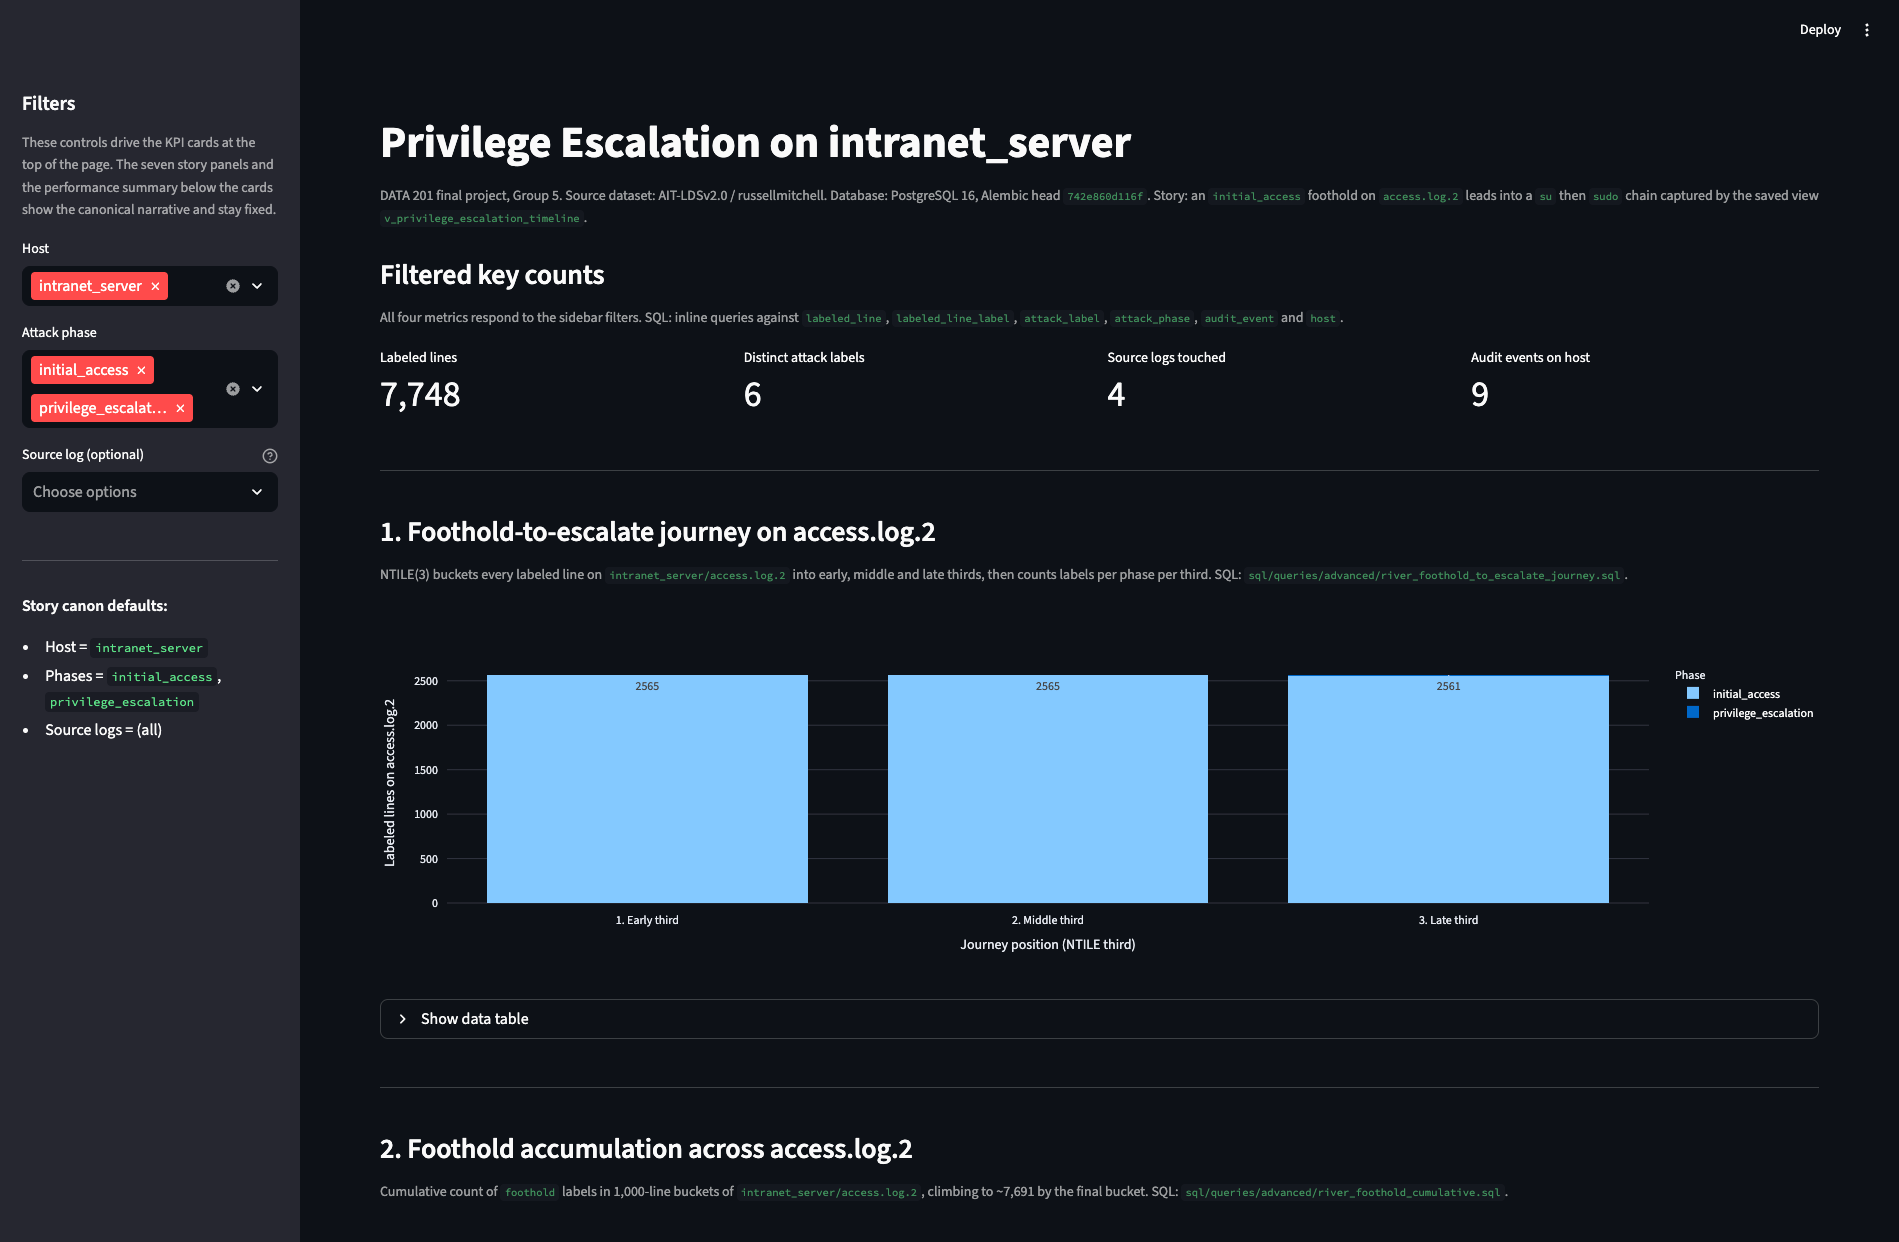
\includegraphics[width=\columnwidth]{figures/dashboard_overview.png}
\caption{Dashboard default view, no filters applied. Eight charts wired
  to the queries in Section~\ref{sec:sql}.}
\label{fig:dashboard-overview}
\end{figure}

\begin{figure}[htbp]
\centering
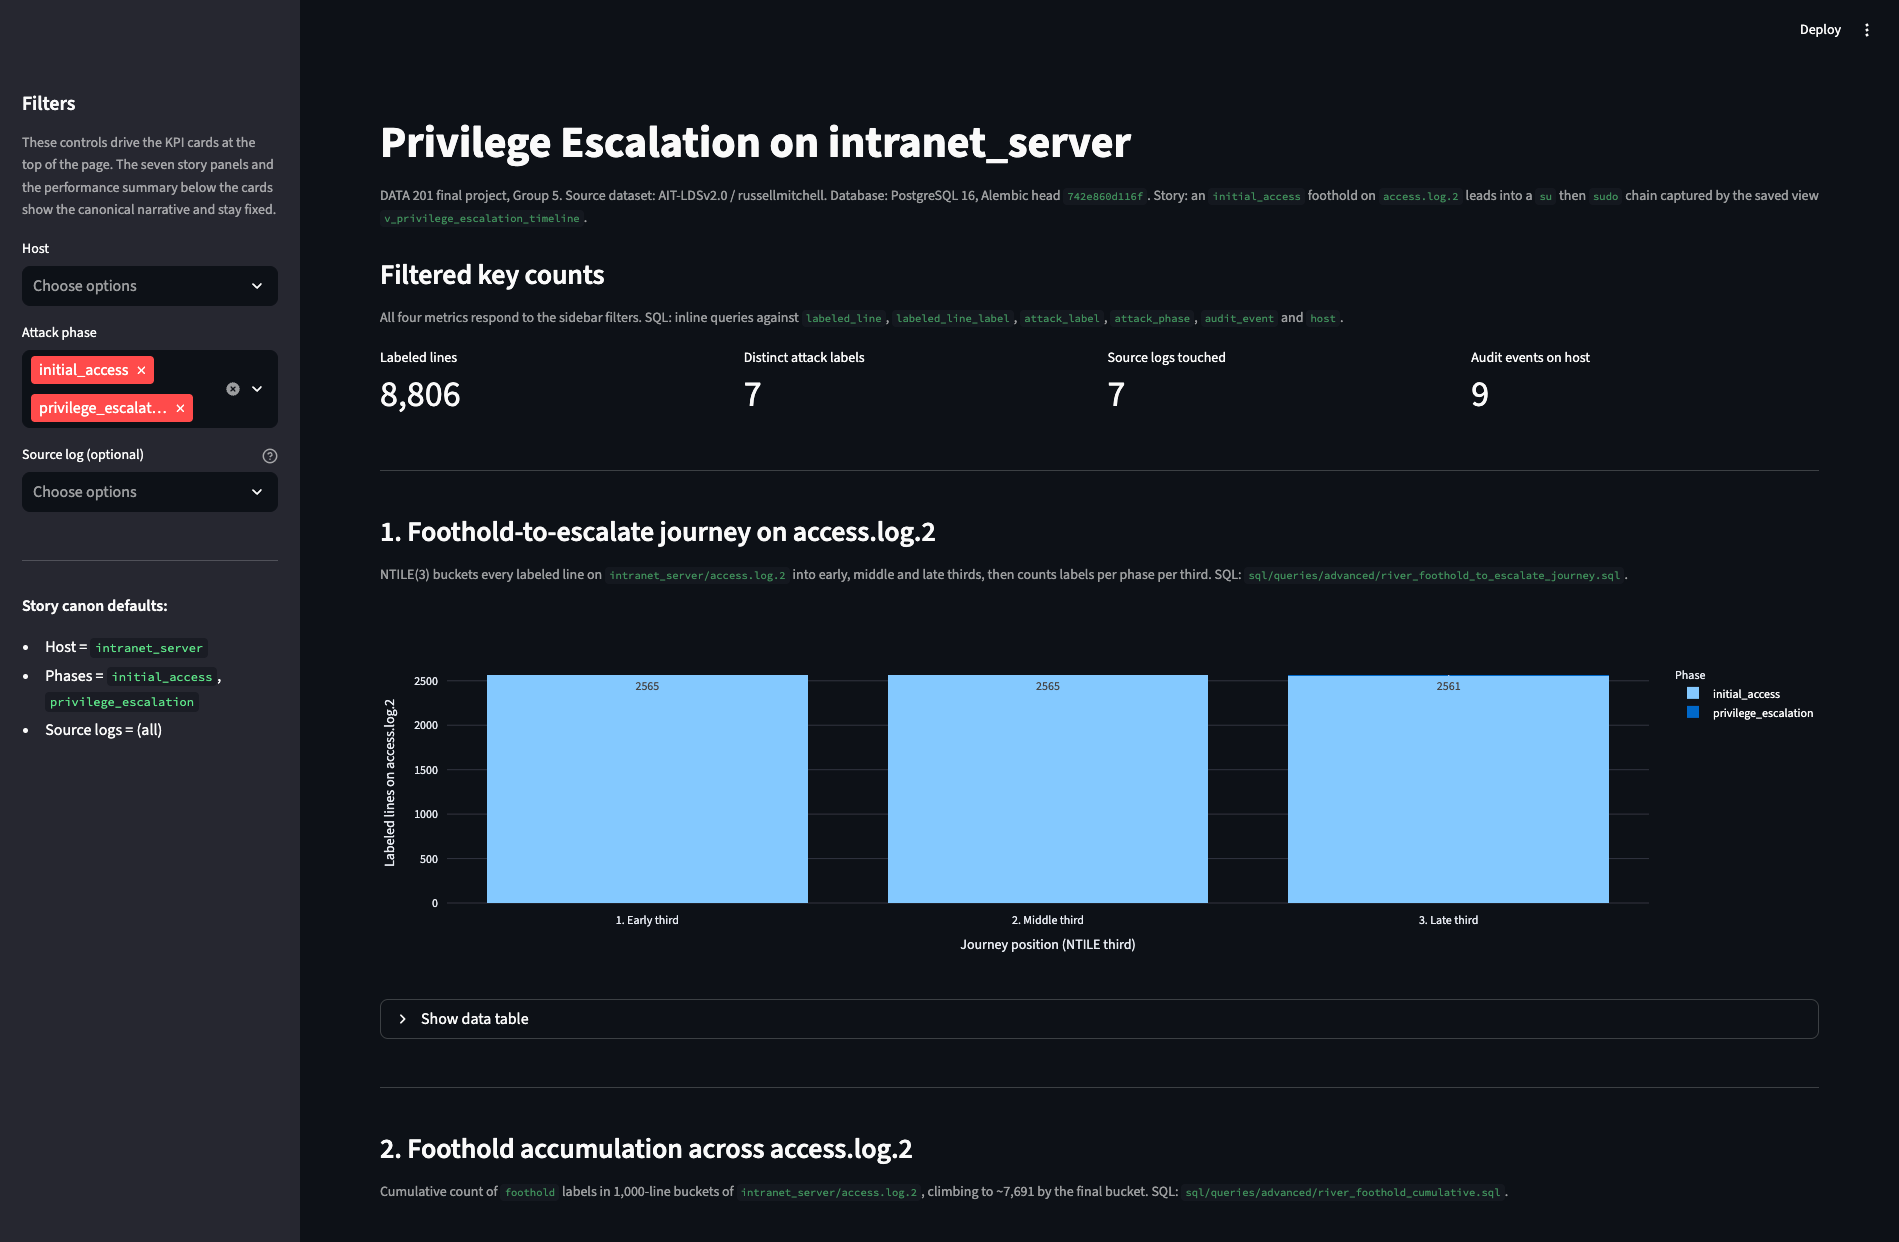
\includegraphics[width=\columnwidth]{figures/dashboard_filter_demo.png}
\caption{Dashboard after filtering to \texttt{intranet\_server}. Charts
  1, 4, 6, 7, and 8 update; charts 2, 3, and 5 (taxonomy / global
  detection-rule volume) are intentionally invariant.}
\label{fig:dashboard-filter}
\end{figure}

\section{Conclusion and Future Work}
\label{sec:conclusion}

\subsection{Findings}
Three findings stand out from the analysis in
Section~\ref{sec:sql}:
\begin{enumerate}
  \item \textbf{Volume is not coverage.} Exfiltration labels dominate
    the corpus by raw line count (roughly 53{,}000 labeled lines),
    but this is an artefact of the DNS-tunneling phase emitting one
    labeled line per DNS query. The privilege-escalation phase has
    only 82 labeled lines but spans five distinct log sources, and
    the operational severity of an account takeover is incomparably
    higher. A detection program optimised for label volume would
    miss the most consequential phase entirely.
  \item \textbf{Cross-source joins are diagnostic.} Queries A4 and
    A6, plus the saved view
    \texttt{v\_privilege\_escalation\_timeline}, reconstruct the
    privilege-escalation sequence and the cross-host lateral movement
    using foreign-key joins between audit events and attack labels.
    Neither view is recoverable from any single log file in
    isolation; the database makes both legible in a single ordering.
  \item \textbf{Timing-only detection is feasible for short bursts.}
    Query A7 uses only \texttt{LAG} over event timestamps and detects
    two distinct attack bursts on \texttt{intranet\_server} without
    consulting a single label. The two-burst structure recovered from
    timing alone matches the structure recovered from labels in
    query A4 exactly. This is a useful unsupervised signal that
    complements rule-based detection.
\end{enumerate}

\subsection{What Happened Next: Exfiltration on \texttt{internal\_share}}
The deck and the report focus on the
\texttt{initial\_access}-into-\texttt{privilege\_escalation} narrative
on \texttt{intranet\_server}, but the dataset's full attack chain
continues for several more hours and migrates to a second host. At
13:50 UTC on the same day (about nine hours after the
\texttt{sudo cat /etc/shadow} burst), \texttt{internal\_share} emits
two audit events for a service called \texttt{put} that starts and
stops within seconds. Query A6 surfaces both events in the same
ordering as the privilege-escalation chain, and the basic
service-activity baseline (B6) confirms that the \texttt{put} service
has no other appearances in the audit data. In the labels domain, the
DNS-tunneling rule \texttt{dnsteal.domain.match} fires roughly
53{,}000 times on the same window, indicating that
\texttt{/etc/shadow} or downstream credentials material was
exfiltrated through DNS queries to the attacker-controlled domain.
The report does not deep-dive the exfiltration phase further: the
loaded slice only contains the audit-domain side of the
exfiltration story, and the more interesting DNS-tunneling channel
lives in a log type that future work will load into the schema (see
Future Work below). The exfiltration phase appears in the dashboard's
KPI band when the user widens the host filter to include
\texttt{internal\_share} and is reproduced in the appendix.

\subsection{Limitations}
\begin{itemize}
  \item \textbf{Single testbed slice.} The current iteration covers
    the \texttt{russellmitchell} testbed only. The other four
    testbeds in AIT-LDSv2.0 share the same schema and could be
    appended with no model changes; the work is loader-only.
  \item \textbf{Out-of-scope log domains.} DNS, OpenVPN, Apache, and
    system auth logs were explored in notebooks but are not loaded
    into the relational schema. Bringing them in would lengthen the
    SQL portfolio (especially for the exfiltration phase) but does
    not change the schema design. The DNS-tunneling channel, in
    particular, is the natural next domain to add: it is the
    highest-line-count phase of the attack and the report currently
    only describes it via the labels domain.
  \item \textbf{Single-machine deployment.} The PostgreSQL container
    runs on one developer machine. The current corpus is small enough
    that this is fine; scaling to the full AIT-LDSv2.0 with all
    testbeds and all log domains would push past a single instance
    and invite the distributed-SQL discussion.
  \item \textbf{Static dashboard scope.} The Streamlit dashboard
    currently shows aggregate views, a filterable timeline, and a
    static EXPLAIN summary. A real SOC dashboard would also support
    time-window scrubbing, alert drill-down, and per-rule
    false-positive review. We treat these as future work rather than
    as gaps.
  \item \textbf{Story-canonical defaults.} The story panels are
    pinned to the \texttt{intranet\_server} narrative so the
    audience does not get lost while experimenting with filters.
    This keeps the dashboard reproducible for grading but means a
    user who wants to investigate a different host has to read the
    SQL and run it manually rather than re-using the UI.
\end{itemize}

\subsection{Future Work}
Concrete and bounded next steps, in order of priority:
\begin{enumerate}
  \item \textbf{Load the remaining four testbeds.} The schema is
    testbed-agnostic; the loader needs a single configuration change
    and an additional run. Brings the labeled corpus from roughly
    62{,}000 to roughly 300{,}000 rows.
  \item \textbf{Add DNS and OpenVPN domains.} The DNS-tunneling
    exfiltration is severely under-represented in the audit-only
    schema. Adding \texttt{dns\_query} and \texttt{vpn\_session}
    tables (with obvious foreign keys to \texttt{host}) would let
    queries like A14 (detection-rule effectiveness) compare
    \texttt{dnsteal.*} rules against audit-based rules on equal
    footing, on the same population.
  \item \textbf{Materialize \texttt{v\_privilege\_escalation\_timeline}.}
    As the corpus grows, the underlying view will become a query-time
    bottleneck. Promoting it to a materialized view with an
    incremental-refresh schedule is a straightforward optimisation
    and provides natural snapshot semantics for the report.
  \item \textbf{Per-host story panels.} The current dashboard pins
    panels 1 to 8 to \texttt{intranet\_server}. Generalising the
    panel SQL so the host filter actually drives the story panels
    (with the privilege-escalation arc replaced by the relevant arc
    for whichever host the user picks) would make the dashboard a
    real investigation tool rather than a curated demo.
  \item \textbf{Productionize the dashboard.} Add user
    authentication, a time-range picker, and a Slack-friendly export
    of the attack timeline. None of these require schema changes.
\end{enumerate}

% Note: The actual reference list is rendered by \bibliography{references}
% in main.tex. This file contains only the AI Use Acknowledgement that the
% rubric requires alongside references.

\section*{AI Use Acknowledgement}

The authors used AI assistants (Anthropic Claude, model
\texttt{claude-opus-4-7}, and OpenAI ChatGPT-5) as drafting and
code-review aides for portions of the SQL queries, the LaTeX skeleton,
and the technical-report prose. Every AI-suggested SQL statement was
independently executed against the project's PostgreSQL database by the
authors; no result reported in this paper is an AI-generated number.
Every analytical claim, schema decision, and trade-off discussion is
the authors' own. The AI assistants did not have access to the
AIT-LDSv2.0 raw data files; data exploration was performed locally in
the notebooks committed under \texttt{notebooks/}.

% TBD adjust to be exactly truthful before submission. If the team used
% additional tools (Cursor, GitHub Copilot, etc.), name them.

\appendix
\section{Collaborative Writing Evidence}
\label{app:collab}

The technical-report rubric (Lecture 11, slide 14) requires the report
to ``show evidence of collaborative writing, not just a final PDF.''
Two artefacts are reproduced here: an Overleaf history snapshot showing
all three authors' colored edit ranges across multiple revisions, and
the project repository's \texttt{git log} restricted to the
\texttt{report/} subtree.

\begin{figure}[htbp]
\centering
% TODO: replace with screenshot from Overleaf -> File -> History
\includegraphics[width=\columnwidth]{figures/overleaf_history.png}
\caption{Overleaf history panel. Each author's edits are rendered in
  a different color. Window covers the period from
  the first \texttt{report/main.tex} commit to the final submission
  on 05/07.}
\label{fig:overleaf-history}
\end{figure}

\begin{figure}[htbp]
\centering
% TODO: replace with terminal screenshot from
%   git log --pretty=format:'%h %an %ad %s' -- report/
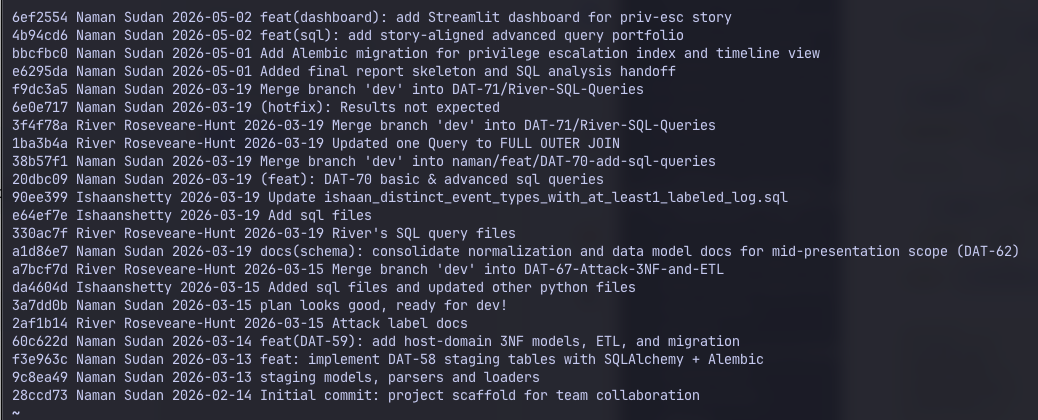
\includegraphics[width=\columnwidth]{figures/git_log_report.png}
\caption{\texttt{git log} restricted to \texttt{report/}. Shows
  contributions from all three authors.}
\label{fig:gitlog-report}
\end{figure}

\section{Repository Map}
\label{app:repo}
The full project repository (frozen at the commit referenced on
Canvas) is laid out as follows:

\begin{verbatim}
data-201-security-log-analysis/
|-- README.md             setup + run + dashboard instructions
|-- docker-compose.yml    Postgres 16
|-- alembic/              schema migrations
|-- src/
|   |-- models/           SQLAlchemy ORM models
|   |-- parsers/          raw log parsers
|   |-- loaders/          ETL pipelines
|   `-- dashboard/        Streamlit app (Section 7)
|-- sql/
|   |-- 3nf/              per-table CREATE TABLE
|   |-- 3nf/_indexes.sql  performance indexes (Section 6.3)
|   |-- 3nf/_views.sql    persisted views (v_attack_timeline)
|   |-- queries/basic/    six basic queries (B1-B6)
|   `-- queries/advanced/ seven advanced queries (A1-A7)
|-- notebooks/            10 exploration notebooks (mid-pres)
|-- docs/
|   |-- schema/           data_model_3nf.md, normalization_raw_to_3nf.md
|   |-- er_diagrams/      drawio sources + exported PDF
|   `-- data_exploration/ per-source findings docs
|-- presentation/         mid-pres + final pres decks
`-- report/               this report (LaTeX sources)
\end{verbatim}


\bibliographystyle{IEEEtran}
\bibliography{references}

\end{document}
